% \iffalse
\let\negmedspace\undefined
\let\negthickspace\undefined
\documentclass[journal,12pt,twocolumn]{IEEEtran}
\usepackage{cite}
\usepackage{amsmath,amssymb,amsfonts,amsthm}
\usepackage{algorithmic}
\usepackage{graphicx}
\usepackage{textcomp}
\usepackage{xcolor}
\usepackage{txfonts}
\usepackage{listings}
\usepackage{enumitem}
\usepackage{mathtools}
\usepackage{gensymb}
\usepackage{comment}
\usepackage[breaklinks=true]{hyperref}
\usepackage{tkz-euclide} 
\usepackage{listings}
\usepackage{gvv}                                        
\def\inputGnumericTable{}                                 
\usepackage[latin1]{inputenc}                                
\usepackage{color}                                            
\usepackage{array}                                            
\usepackage{longtable}                                       
\usepackage{calc}                                             
\usepackage{multirow}                                         
\usepackage{hhline}                                           
\usepackage{ifthen}                                           
\usepackage{lscape}
\usepackage{amsmath}
\usepackage{caption}
\newtheorem{theorem}{Theorem}[section]
\newtheorem{problem}{Problem}
\newtheorem{proposition}{Proposition}[section]
\newtheorem{lemma}{Lemma}[section]
\newtheorem{corollary}[theorem]{Corollary}
\newtheorem{example}{Example}[section]
\newtheorem{definition}[problem]{Definition}
\newcommand{\BEQA}{\begin{eqnarray}}
\newcommand{\EEQA}{\end{eqnarray}}
\newcommand{\define}{\stackrel{\triangle}{=}}
\theoremstyle{remark}
\newtheorem{rem}{Remark}
\begin{document}

\bibliographystyle{IEEEtran}
\vspace{3cm}

\title{NCERT 10.5.3 10Q}
\author{EE22BTECH11010 - Venkatesh D Bandawar $^{*}$% <-this % stops a space
}
\maketitle
\newpage
\bigskip

\renewcommand{\thefigure}{\theenumi}
\renewcommand{\thetable}{\theenumi}

\parindent 0px
\textbf{Question:} Show that $a_0$ , $a_1$ , $a_2$
, . . ., $a_n$
, . . . form an AP where an is defined as below :
\begin{enumerate}
    \item $a_n$ = $(3 + 4n)$ 
    \item $a_n$ = $(9 - 5n)$ 
\end{enumerate}
Also find the sum of the first 15 terms in each case.

\vspace{0.5cm}
\textbf{Answer:} 
\begin{enumerate} [label=(\roman*)]
    \item We know that, The AP has constant common difference between two consecutive terms.
    \begin{align}
        \therefore \text{common difference } (d) &= a_{n+1} - a_n \\
        &= \brak{3+4\brak{n+1}} \nonumber\\
        & u\brak{n+1} -\brak{3+4n}u\brak{n} \nonumber\\
        &= 4
    \end{align}
   $\because$ Given equation has common difference between any two consecutive terms is $4$ i.e. independent of '$n$'\\
    Hence given sequence is in AP.
    \begin{table}[htbp] 
    \centering
    \begin{tabular}{|c|c|c|}
\hline
    Parameter & Description & Value\\
    \hline
    $P(s)$ & Plant Transfer Function & $\frac{0.001}{s\brak{\frac{s}{0.5}+1}\brak{\frac{s}{100}+1}}$\\
    \hline
    $C(s)$ & Lag Compensator  & $\frac{100\brak{\frac{s}{10}+1}}{\frac{s}{0.1}+1}$\\
    \hline
    $T(s)$ & Loop gain  & $P(s) C(s)$ \\
    \hline
    $\omega$ & Angular Frequency & 3rad/s \\
    \hline
\end{tabular}

    \caption{\normalsize\textsl{Given \, parameters in $1^{st}$ AP}}
    \label{given parameters list}
    \end{table}

    \begin{align}
         X(z) &= \sum_{n = -\infty}^{\infty} x(n) z^{-n} \label{eq:z-transform}\\
        \implies  X(z) &= \sum_{n = -\infty}^{\infty}[3 + 4n].u(n) \, z^{-n} \\
        nu(n) &\system{Z} -z.U'(z)\\
        \implies X(z) &= \frac{3}{1-z^{-1}} + \frac{4.z^{-1}}{(1-z^{-1})^2} ; |z|>1\\
        \because y(n) &= x(n) * u(n)\\
        y(n) &\system{Z} Y(z) \nonumber\\
        \implies Y(z) &= \left[ \frac{3}{1-z^{-1}} + \frac{4 z^{-1}}{\left(1-z^{-1}\right)^2} \right].\frac{1}{1-z^{-1}}
    \end{align}
    Using contour integeration for inverse Z transformation,\\
    \begin{align}
        y(14) &= \frac{1}{2\pi j}\int Y(z) z^{13} dz \\
        y(14) &= \frac{1}{2\pi j}\int \frac{3.z^{15}}{(z-1)^{2}} dz + \frac{1}{2\pi j}\int \frac{4.z^{15}}{(z-1)^{3}} dz\\
        \because R&=\frac{1}{\brak {m-1}!}\lim\limits_{z\to a}\frac{d^{m-1}}{dz^{m-1}}\brak {{(z-a)}^{m}f\brak z}\\
        R_1 &=\frac{1}{1!}\lim\limits_{z\to 1}\frac{d}{dz}\brak {(z-1)^2.\frac{3.z^{15}}{(z-1)^{2}}}\\
        R_1 &= 45\\
        R_2 &=\frac{1}{2!}\lim\limits_{z\to 1}\frac{d^2}{dz^2}\brak {(z-1)^3.\frac{4.z^{15}}{(z-1)^{3}}}\\
        R_2 &= 420\\
        \implies y(14) &= R_1 + R_2 \nonumber\\
        &= 465
    \end{align}
    
    \begin{figure}[!h] 
    \centering
    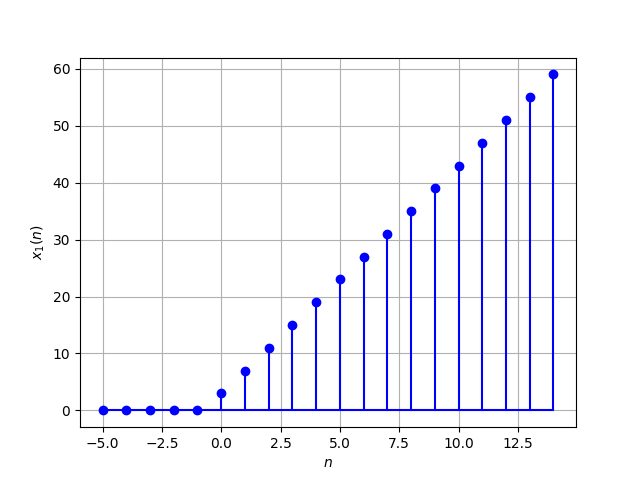
\includegraphics[width=\columnwidth]{figs/signal_x1.png}
    \caption{$x_1(n)=(3+4n)u(n)$}
    \label{fig:Graph1}
    \end{figure}
    
    \item We know that, The AP has constant common difference between two consecutive terms.
    \begin{align}
        \therefore \text{common difference } (d) &= a_{n+1} - a_n  \\
        &= \brak{9-5(n+1)}u\brak{n+1} \nonumber\\
        &- \brak{9-5n}u\brak{n} \nonumber\\
        &= -5
    \end{align}
   $\because$ Given equation has common difference between any two consecutive terms is $-5$ i.e. independent of '$n$'
   \begin{center}
       Hence given sequence is in AP.
   \end{center}

    \begin{table}[htbp] 
    \centering
    \begin{tabular}{|c|c|c|c|}
\hline
\textbf{Parameter}&\textbf{Description} &\textbf{subquestion}& \textbf{Value}\\
\hline
     \multirow{4}{*}{$\Delta \theta$} & \multirow{4}{*}{$\theta_1 - \theta_2$} &\brak{a}& 6.4$\pi$ \, radians \\
     \cline{3-4}
     & & \brak{b}& 0.8$\pi$ \, radians \\
     \cline{3-4}
     & &\brak{c}& $\pi$ \, radians \\
     \cline{3-4}
     & & \brak{d} & $\dfrac{3\pi}{2\vphantom{\brak{0.1}}}$ \, radians \\
     \hline
\end{tabular}

    \caption{\normalsize\textsl{Given \, parameters in $2^{st}$ AP}}
    \label{given parameters list}
    \end{table}

    \begin{align}
         X(z) &= \sum_{n = -\infty}^{\infty} x(n) z^{-n} \label{eq:z-transform}\\
        \implies  X(z) &= \sum_{n = -\infty}^{\infty}[9 - 5n].u(n) \, z^{-n} \\
        nu(n) &\system{Z} -z.U'(z)\\
        \implies X(z) &= \frac{9}{1-z^{-1}} - \frac{5.z^{-1}}{(1-z^{-1})^2} ; |z|>1\\
        \because y(n) &= x(n) * u(n)\\
        y(n) &\system{Z} Y(z) \nonumber\\
        \implies Y(z) &= \left[ \frac{9}{1-z^{-1}} - \frac{5 z^{-1}}{\left(1-z^{-1}\right)^2} \right].\frac{1}{1-z^{-1}}
    \end{align}
    Using contour integeration for inverse Z transformation,\\
    \begin{align}
        y(14) &= \frac{1}{2\pi j}\int Y(z) z^{13} dz \\
        y(14) &= \frac{1}{2\pi j}\int \frac{9.z^{15}}{(z-1)^{2}} dz - \frac{1}{2\pi j}\int \frac{5.z^{15}}{(z-1)^{3}} dz\\
        \because R&=\frac{1}{\brak {m-1}!}\lim\limits_{z\to a}\frac{d^{m-1}}{dz^{m-1}}\brak {{(z-a)}^{m}f\brak z}\\
        R_1 &=\frac{1}{1!}\lim\limits_{z\to 1}\frac{d}{dz}\brak {(z-1)^2.\frac{9.z^{15}}{(z-1)^{2}}}\\
        R_1 &= 135\\
        R_2 &=\frac{1}{2!}\lim\limits_{z\to 1}\frac{d^2}{dz^2}\brak {(z-1)^3.\frac{5.z^{15}}{(z-1)^{3}}}\\
        R_2 &= 525\\
        \implies y(14) &= R_1 - R_2 \nonumber\\
        &= -390
    \end{align}
    
    \begin{figure}[!h] 
    \centering
    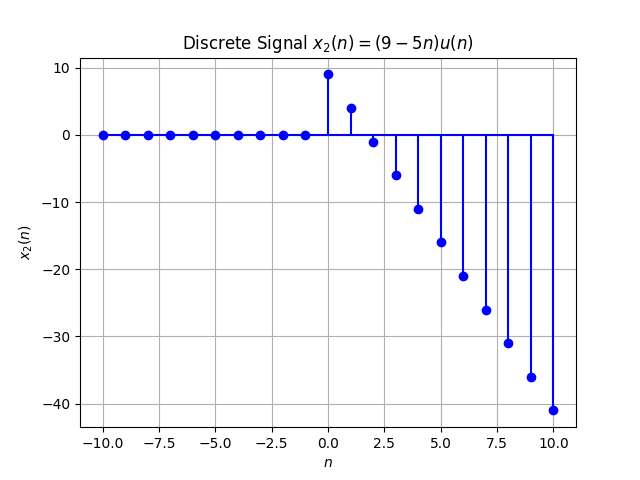
\includegraphics[width=\columnwidth]{figs/signal_x2.png}
    \caption{$x_2(n)=(9-5n)u(n)$}
    \label{fig:Graph2}
    \end{figure}

\end{enumerate}

\end{document}
